\chapter[To Be Figured Out]{To Be Figured Out: Inductive Bias, Non-Stationarity
  and Linear Recurrence}
\label{ch:07-to-be-figured-out}
\chaptermark{To Be Figured Out}

\lecturemeta{Razvan Pascanu}{Mila and Google DeepMind}

The title above is the deck's own, and it is accurate: this is a survey of open problems rather
than a result. Its spine is an argument about inductive bias: there is no prior-free machine learning system, every choice
in building one is a bias, and the useful question is therefore not whether to have biases but
which ones buy the most. Pascanu develops that in three registers. Conceptually, the i.i.d.\
assumption is itself a bias doing hidden work, because gradient descent resolves credit assignment
by a tug-of-war between examples and that only works when the data is shuffled. Structurally,
depth and architecture are biases with quantifiable payoffs. Practically, state space models and the
linear recurrent unit buy capability from structure instead of scale, and by the end most of that advantage has evaporated into a hybrid.

\section*{Key ideas}

\paragraph{Why look beyond i.i.d.\ at all.} Four reasons, none of them about benchmark scores.
Scaling is unsustainable, argued with data-centre water and electricity figures rather than
FLOPs. The world is bigger than the agent: models have finite capacity, the world is large and
includes the people modelling it, so continual learning is in a sense unavoidable. Learning on
the fly reframes the goal from asymptotic performance to a tracking question, how well can we
follow a moving target, which makes trade-offs such as compute against performance and
robustness against performance explicit. And efficiency of learning, via
Griffiths~\citep{griffiths2020}: the profile of human intelligence is a consequence of human
limitations, and AlphaGo's move 37 was available precisely because the machine does not
decompose problems into tractable subproblems the way people do, sacrificing performance for
efficiency. Pascanu's hypothesis is that trade-offs are necessary and that limitations should
be exploited to shape the loss surface.

\paragraph{The i.i.d.\ assumption is doing hidden work.} Gradient-based credit assignment inside a
function approximator proceeds by
tug-of-war dynamics between competing examples, which requires the data to be i.i.d. Two consequences are offered as hypotheses, not facts: there is no explicit knowledge
composition, and scale becomes a crutch that makes learning possible at all. Failure of credit
assignment is then what catastrophic forgetting \emph{is}, rather than a separate phenomenon.
The natural inference, that curricula should therefore help, does not survive
contact~\citep{schaul2019, toneva2019}, and the lecture explains why exploiting this is not
easy: we do not know how to measure what we care about when building a representation, and
learning lacks compositionality and locality.

\paragraph{No prior-free learning, and depth as a quantifiable prior.} Priors, regularisers
and inductive biases all restrict or reshape the search space, and since every step in
constructing a system is such a choice, the King Midas framing is that the choice cannot be
declined. Depth is the cleanest example of a bias with a countable payoff: Zaslavsky's
theorem on hyperplane arrangements~\citep{zaslavsky1975} bounds how a single layer partitions
input space, and composing layers multiplies regions, which is the counting argument behind
the number of linear regions of a deep network~\citep{montufar2014}. On optimisation the
lecture is deflationary about the folklore. High-dimensional non-convex loss surfaces are
dominated by saddles rather than bad minima~\citep{dauphin2014}, so the deep learning myth,
that networks can be dropped in anywhere and optimisation behaves as if convex, holds only if
the right protocol is used. Initialisation and the choice of optimiser qualitatively alter which
solution is reached, which Pascanu argues should be leveraged instead of treated as
nuisance; and a loss surface of sufficient dimension contains every low-dimensional
pattern~\citep{czarnecki2019}, which is a warning about reading too much into loss-landscape
visualisations.

\begin{figure}[htbp]
\centering
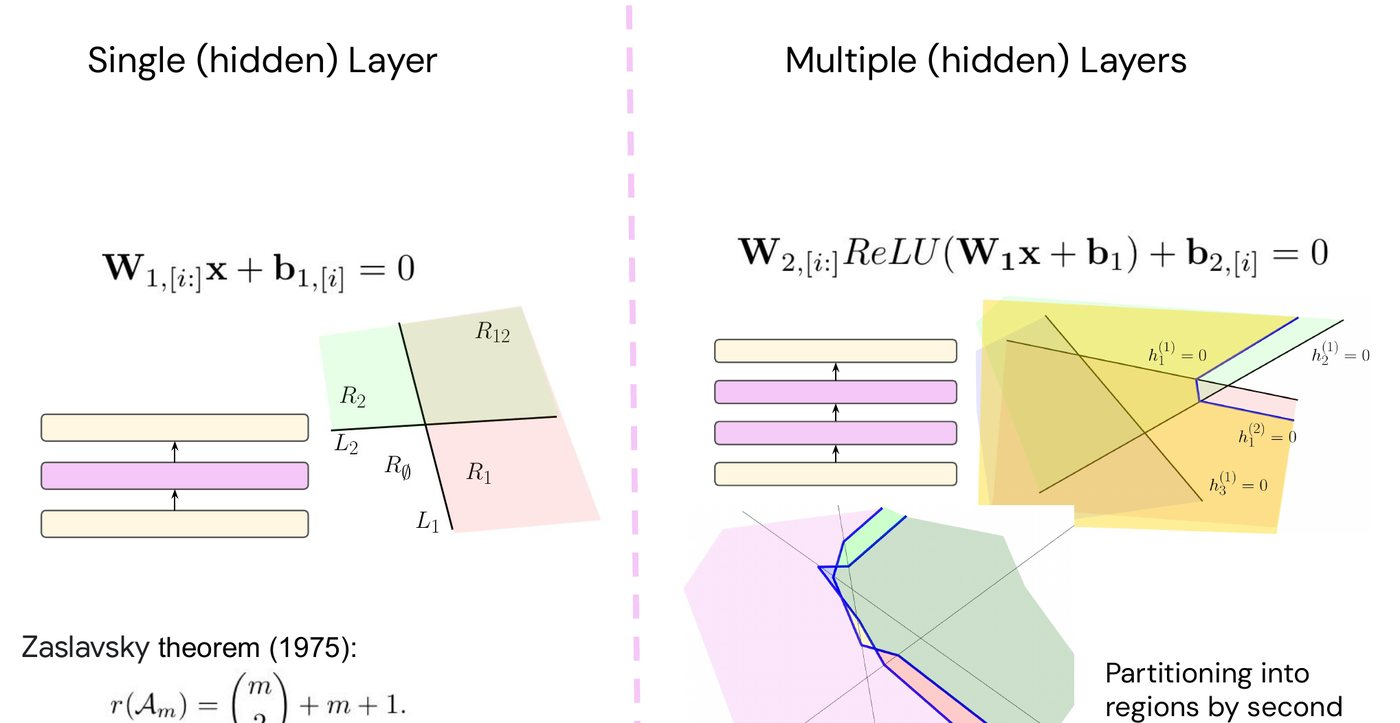
\includegraphics[width=0.80\textwidth]{figures/to-be-figured-out-2.jpg}
\caption{Depth as a bias with a countable payoff, from the To Be Figured Out lecture. A single hidden
layer cuts input space with hyperplanes $\mat{W}_{1,[i:]}\xin + \vect{b}_{1,[i]} = 0$, and
Zaslavsky's formula gives the number of resulting regions. A second layer's boundaries
$\mat{W}_{2,[i:]}\,\mathrm{ReLU}(\mat{W}_1\xin + \vect{b}_1) + \vect{b}_{2,[i]} = 0$ are
piecewise linear, bending as they cross the first layer's regions, so the count multiplies
rather than adds. This is the origami picture of why depth buys expressivity.}
\label{fig:to-be-figured-out-2}
\end{figure}

\paragraph{State space models, and why they are hard to reason about.} The second half opens
with a hardware question: are transformers optimal? The worry is inference cost, usually framed
as the quadratic cost of attention, and the comparison the lecture draws is per-step: recurrence
is $O(1)$, attention $O(N)$. State space models are the community's main answer, and Pascanu
describes them as a variant of linear RNNs. An SSM models the sequence in continuous time,
relies on a deterministic HiPPO initialisation, and is then discretised; the payoff is that the
discretised system can be read either as a recurrence, which makes inference fast, or as a
convolution, which makes training fast. That dual view is the whole appeal.

His objection is methodological, not empirical. There are many variants (S4~\citep{gu2022s4},
S4D, H3, Mamba~\citep{gu2023mamba}), several discretisation schemes such as bilinear and
zero-order hold, it is unclear how changes to the surrounding block interact with the SSM's
parameterisation, and for the better-performing SSMs the continuous-time story becomes
strenuous. The question he poses is how to disentangle which ingredient is actually doing the
work.

\paragraph{The LRU as an ablation, not a new model.} The linear recurrent unit is the answer to
that question, derived in six steps~\citep{orvieto2023}. Start from a transformer backbone,
because the MLP supplies the expressivity and therefore the recurrent block is allowed to be
simple. Remove the nonlinearity from the recurrence, which costs less than expected: linear
RNNs followed by nonlinear projections can approximate any finite sequence-to-sequence map, with
the linear recurrence compressing the sequence and the MLP approximating the decompressor. The
caveat is stated, that this construction can only exhibit fading memory. Linearity then permits
diagonalisation, so a complex diagonal $\Lam$ is learned directly and the recurrent computation
collapses, and stability becomes a statement about eigenvalues: inside the unit disk gives
exponentially decaying sine waves, outside is unstable. Vanishing gradients are the mirror
image, since eigenvalues near the origin decay within a few steps, so initialisation samples an
annulus that excludes the origin, typically $r_{\min} = 0.9$ and $r_{\max} = 0.999$
(Figure~\ref{fig:to-be-figured-out-1}). Stable parameterisation and normalisation, the latter
needed to control hidden-state growth, complete the recipe.

The results that matter here are the negative ones. HiPPO is not necessary. Continuous time is
not necessary. Complex numbers may be doing nothing more than providing a compact
representation, since a symmetric real system can perform similar computations at the cost of a
larger state. In other words, most of the conceptual apparatus that SSM papers carry is
detachable, and what remains is a diagonal linear recurrence with a sane spectrum. The lecture
then descends to hardware, noting a roughly eightfold gap between HBM and VMEM transfer rates on
the TPU profiled, and that a linear RNN performs an associative scan and so parallelises across
time despite being a recurrence.

\begin{figure}[htbp]
\centering
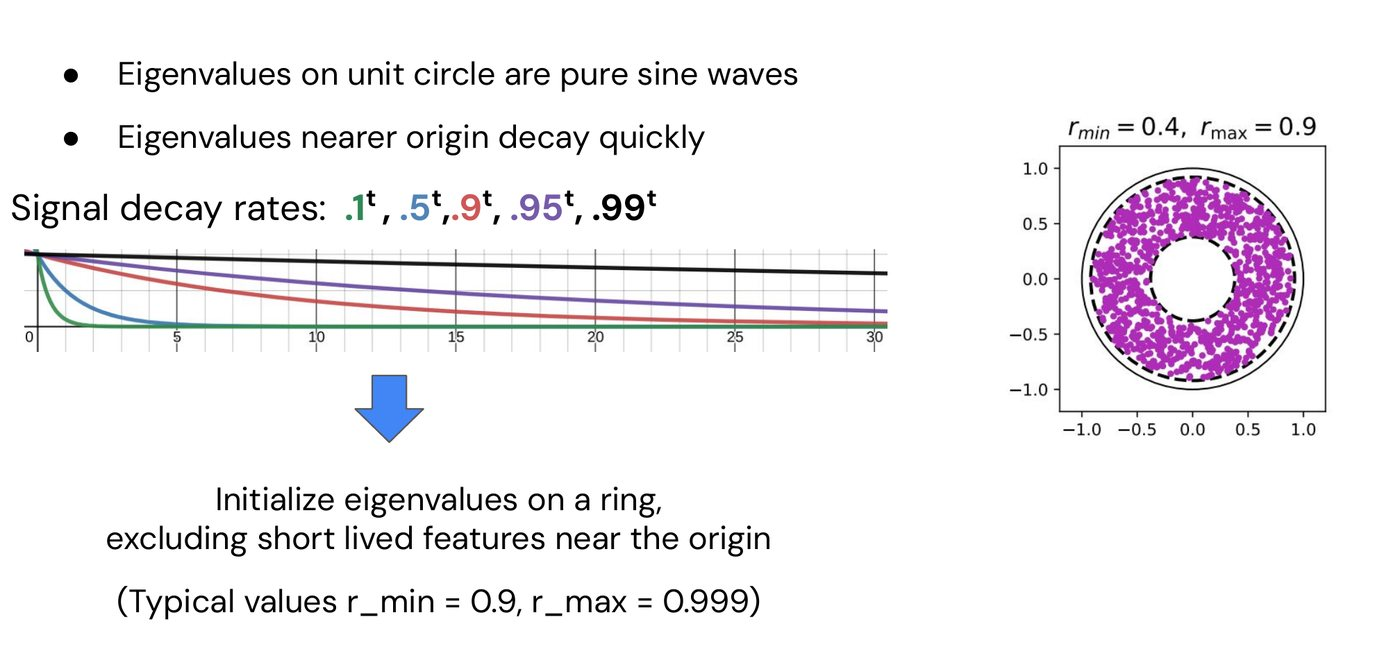
\includegraphics[width=0.82\textwidth]{figures/to-be-figured-out-1.jpg}
\caption{Step three of the linear recurrent unit derivation, from the To Be Figured Out
lecture. Left, signal decay $r^{t}$ for $r$ from $0.1$ to $0.99$: an eigenvalue of modulus
$0.5$ has effectively forgotten its input within five steps, while $0.99$ persists past thirty.
Right, the consequence for initialisation, eigenvalues sampled from an annulus rather than a
disk so that no unit starts with a memory too short to be useful. The annulus drawn uses
$r_{\min} = 0.4$, $r_{\max} = 0.9$; the values recommended in practice are $0.9$ and $0.999$.}
\label{fig:to-be-figured-out-1}
\end{figure}

\paragraph{The scorecard, and the hybrid that actually wins.} Having built the case,
Pascanu reports that pure recurrence does not straightforwardly win. On language S4D did not work
out of the box and an LSTM was better; gating it helped. What does work is a hybrid, and the
reasoning is that SSMs and linear attention share the two properties that matter, a finite state
and linear scaling in sequence length, while being complementary in what they capture: the SSM
models the whole sequence, linear attention captures local information. The recipe given is a
block pattern repeating two SSM blocks to one linear-attention block, and the configuration
reported as state of the art at scale is roughly 75\% linear attention with 25\% global softmax
attention retained (Figure~\ref{fig:to-be-figured-out-3}). As models scale, behaviour and
limitations converge, so the remaining gains are situational: online inference, and scaling down
by distillation. The closing summary keeps
both halves: biases are unavoidable, continual learning may be the next change of perspective,
scale might work but is not the only option, transformers rely on a factorisation of simple
components that must be scaled, and attention might not be all we need.

\begin{figure}[htbp]
\centering
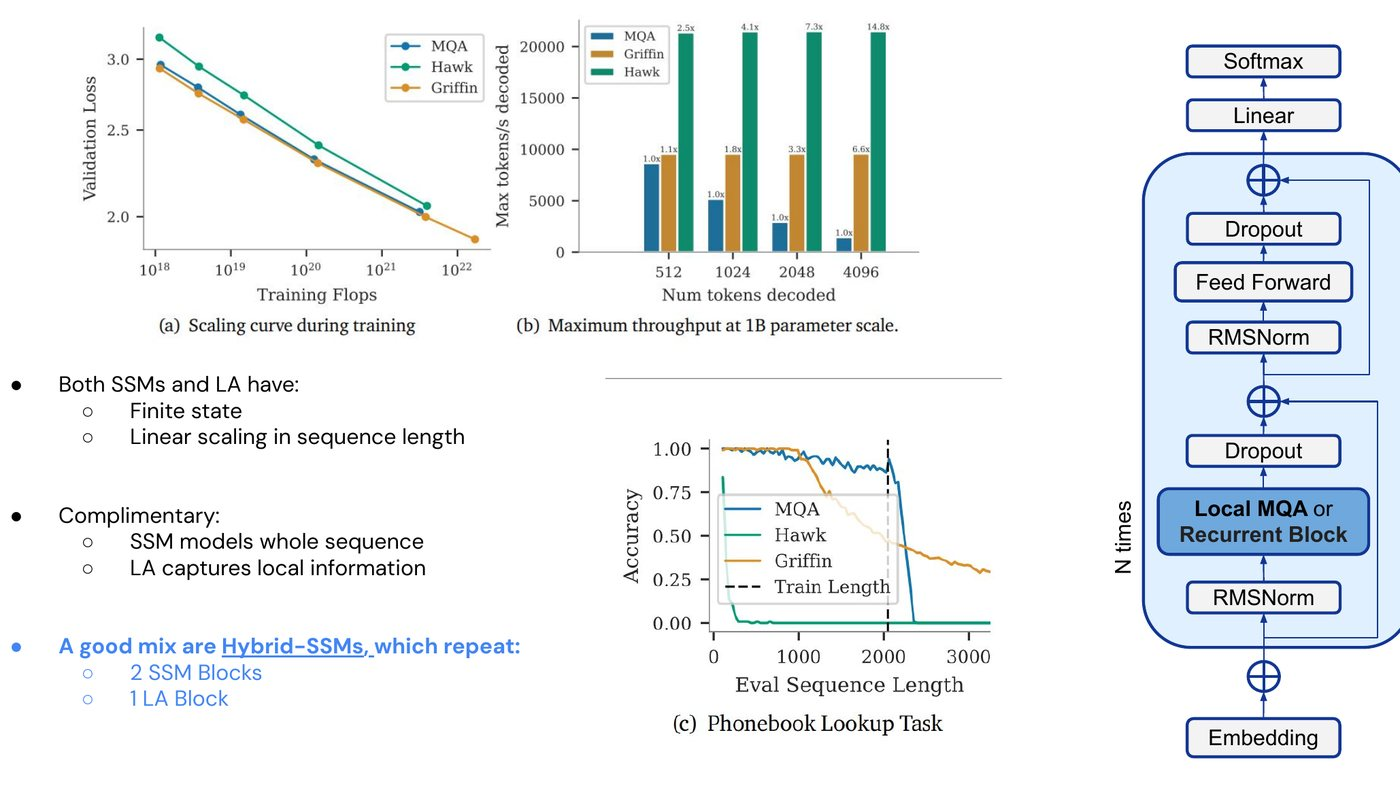
\includegraphics[width=0.86\textwidth]{figures/to-be-figured-out-3.jpg}
\caption{What actually wins, from the To Be Figured Out lecture. Left, the case for hybrids:
state space models and linear attention share a finite state and linear scaling in sequence
length, and are complementary because the SSM models the whole sequence while linear attention
captures local structure. Middle, the evidence, with matched scaling curves, an order-of-magnitude
throughput advantage at 1B parameters, and a phonebook-lookup task where the pure recurrent
variants degrade past their training length. Right, the resulting block, alternating a recurrent
or local-attention block with feed-forward layers.}
\label{fig:to-be-figured-out-3}
\end{figure}

\section*{Notation}

$\Lam$ denotes the diagonal matrix of recurrence eigenvalues, $r$ their modulus, $t$ discrete
time. The lecture uses $\theta$ for parameters as elsewhere in this book, and writes
$\theta_0$, $\theta_{\text{generalize}}$ and $\theta_{\text{overfit}}$ for points in parameter
space when discussing capacity, which is retained here in prose rather than symbols.

\section*{Why it matters}

Read this immediately after Chapter~\ref{ch:06-continual-learning}, because Lyle and Pascanu
disagree in an interesting way. Lyle treats plasticity loss as a set of fixable engineering
faults in the optimiser and the architecture; Pascanu treats the same territory as evidence
that gradient-based credit assignment is structurally dependent on i.i.d.\ data, which is a
much stronger claim and would mean the fixes are palliative. The linear-recurrence material
also connects to Chapter~\ref{ch:10-efficient-learning}: both lectures end up at the same
place, that the binding constraint is memory bandwidth rather than arithmetic, and both reach it
from opposite directions. The personal note to ``check the MAMBA paper'' belongs
here~\citep{gu2023mamba}, with the caution that Pascanu's point is precisely that Mamba's
continuous-time framing is not what makes it work.

\begin{aside}
Pascanu's deck borrows three slides from Kyunghyun Cho on language modelling, and cites the
statistics view that firing a linguist improves the recogniser. Set against
Chapter~\ref{ch:05-statistics-estimation}, where Cho argues for learning the estimator rather
than modelling the process, the two speakers are making the same argument from different ends:
Cho says the generative process need not be modelled, Pascanu says some prior about it is
unavoidable. Both are right, and what is left over is the question of which biases are cheap to
state and expensive to learn.
\end{aside}
